\subsection{Evaluaci\'on final del desempe\~no del software 1}
    Para la evaluaci\'on del desempe\~no, en esta ocasi\'on fue
        mucho m\'as claro la medida del tiempo transcurrido entre el
        paso de una generaci\'on y otra, y esto es debido al tama\~no en
        el cual crece el arreglo de dimensi\'on $n * n$, ya que mientras
        se tenga un $n$ mucho m\'as alto, el rango de evaluaci\'on
        tambi\'en crece considerablemente y tambi\'en lo hacen las
        evaluaciones en cada una de las c\'elulas, donde las reglas del
        algoritmo del Physarum deben de hacer posible la transici\'on
        entre cada uno de los estados.
    \vskip 0.5cm
    A continuaci\'on, se muestran algunas de las configuraciones
    junto con sus resultados y los datos recopilados en tama\~nos
    mucho m\'as extensos:
    \vskip 0.5cm
    %figura
    \begin{figure}[htbp]
        \centering
        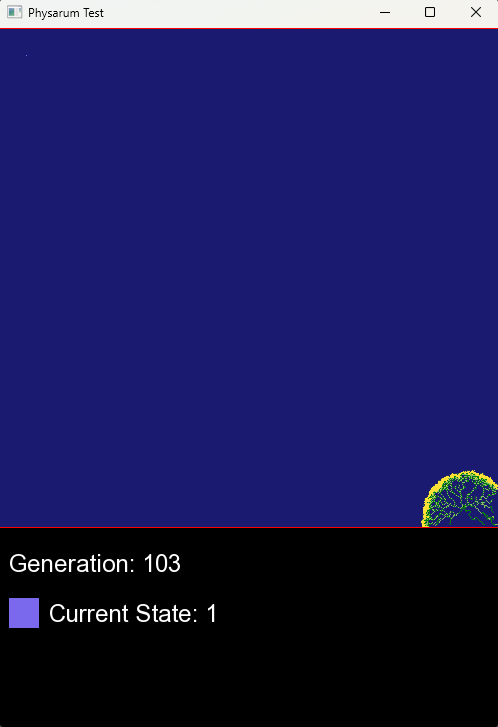
\includegraphics[width=0.5\textwidth]{./images/Pruebas/simulador/image079.png}
        \caption{Expansi\'on y evaluaci\'on de la simulaci\'on en un entorno mucho mas grande (500 x 500)}
        \label{fig:Ruta 79}
    \end{figure}
    \vskip 0.5cm
    %figura
    \begin{figure}[htbp]
        \centering
        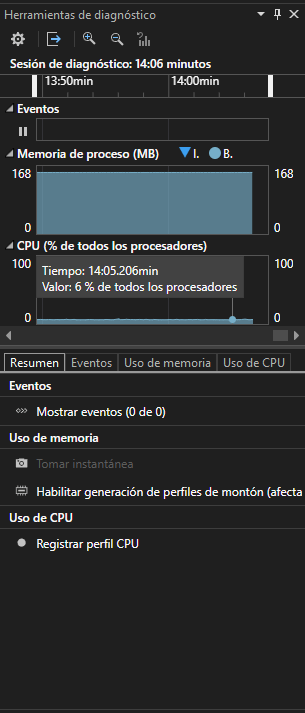
\includegraphics[width=0.5\textwidth]{./images/Pruebas/simulador/image080.png}
        \caption{Cantidad de memoria y procesamiento durante la ejecu\'on del simulador}
        \label{fig:Ruta 80}
    \end{figure}
    \vskip 0.5cm
    %figura
    \begin{figure}[htbp]
        \centering
        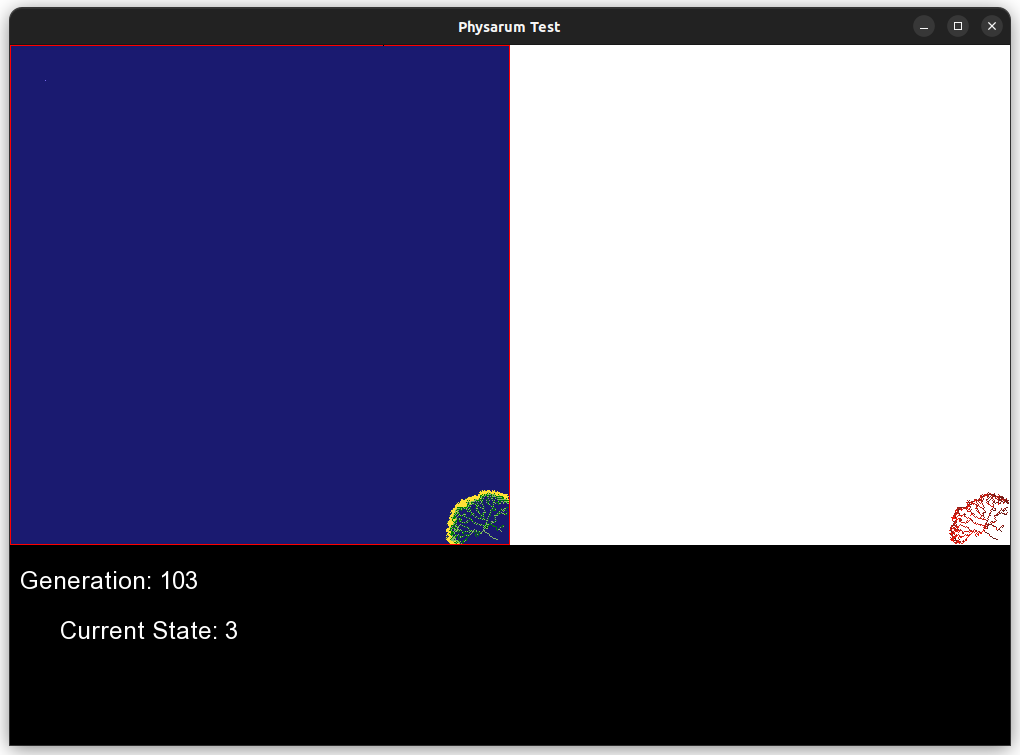
\includegraphics[width=0.5\textwidth]{./images/Pruebas/simulador/image081.png}
        \caption{Expansi\'on en el mismo tama\~no del que fue realizado en Linux.}
        \label{fig:Ruta 81}
    \end{figure}
    \vskip 0.5cm
    %figura
    \begin{figure}[htbp]
        \centering
        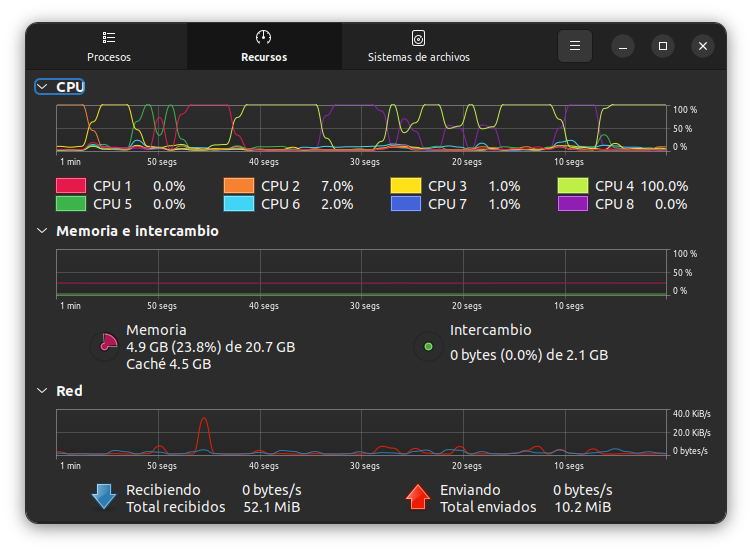
\includegraphics[width=0.5\textwidth]{./images/Pruebas/simulador/image083.png}
        \caption{Uso de los recursos del computador durante la ejecuci\'on del simulador.}
        \label{fig:Ruta 83}
    \end{figure}
    \vskip 0.5cm
    La evaluaci\'on final del desempe\~no del software se centr\'o en
        medir el tiempo de simulaci\'on y la precisi\'on de las rutas
        generadas bajo diversas condiciones iniciales y sistemas
        operativos. Se comprob\'o que el algoritmo, aunque eficiente
        en la mayor\'ia de los casos, presenta diferencias de
        desempe\~no notables entre Windows y Linux, con mejores
        resultados en Linux debido a su mayor capacidad de
        procesamiento en simulaciones intensivas.
    \vskip 0.5cm
    El an\'alisis de los tiempos de ejecuci\'on entre una generaci\'on
        y la siguiente permiti\'o identificar mejoras clave en la
        eficiencia del software. Los resultados mostraron que, en
        entornos de mayor complejidad, el tiempo de procesamiento
        incrementa proporcionalmente al n\'umero de barreras y
        obst\'aculos, lo que requiere optimizaciones adicionales en
        futuras iteraciones.